\documentclass[11pt]{article}
%Gummi|065|=)
\usepackage{listings}
\lstset{language=C}
\usepackage[utf8]{inputenc}
\usepackage[T1]{fontenc}
\usepackage{epstopdf}
\usepackage{lmodern}
\usepackage{amsmath}
\usepackage{geometry}
\usepackage{color}
\usepackage{xcolor}
\usepackage{listings}
\usepackage{graphicx}

\usepackage{caption}
\geometry {a4paper, top=25mm, left=25mm, right=25mm, bottom=25mm}
\DeclareCaptionFont{white}{\color{white}}
\DeclareCaptionFormat{listing}{\colorbox{gray}{\parbox{\textwidth}{#1#2#3}}}
\captionsetup[lstlisting]{format=listing,labelfont=white,textfont=white}
\title{\textbf{Parallel Computig Report: 2d Stencil Computation}}
\author{Mihail Bogojeski\\
		Armin Puffler}
\date{}
\begin{document}

\maketitle

\section{Problem Statement}

The problem we are to work on consists of a parallel 2-d stencil computation.\\
Given an $n \times m$ matrix, with boundary conditions given in 4 vectors, we are to iterate over the matrix and update every field for a given number of iterations.\\ 
The update function consists of a given function $f$ which computes the value of the cell $c$ by taking the average value of its 'Von Neumann neighborhood'. In essence this operation is identical to '2D Jacobi Iteration'.\\
This operation is not trivial since once a cell is updated, it can no longer be used by the next cell to compute its average. Performance and memory optimizations are thus slightly hindered.\\
 
\section{Hypothesis}

We want to show that there are different approaches to solving this problem, not every one of them has the same efficiency though. We are comparing varying versions of a few basic methods, while demonstrating that column- and diagonal-based traversions of a matrix do not intertwine readily with the buffer-system of the programming language we are basing this experiment on.

\section{Explanation of the algorithms: 2D-Stencil Computation: }

The basic algorithm is simple: The matrix (e.g.: each cell of the matrix) is iteratively being updated by a function as until some condition is met. In this case, we have a certain count of iterations that must be fulfilled until the program is to terminate.
The function $f$ that carries out said update on a cell $c$, defined by coordinates $x, y$ takes the 4 Neumann neighbors and determines its average:



\[  f(x, y) = \frac{a_{(x-1)y} + a_{x_+1)y} + a_{x(y+1)} + a_{x(y-1)}}{4}  \]



\section{MPI framework implementation}

For our MPI implementation we made 4 versions of the program to test how 4 different approaches at communication work and how they affect the speedup.
The initialization and finalization part of all programs is the same. The main idea behind the algorithm is to split the matrix into $p$ submatrices and assign
each processor a submatrix. Each process then iterates and update the submatrix locally, only communicating with each neighbour once per iteration, in order to
get the updated version of its boundaries.//
\subsection{Initialization and finalization}
The whole matrix is first initialized only by the first process, and left NULL in all others.
Then, each process creates and initializes its own submatrix. Both the matrix and submatrix are allocated as a single one-dimensional array. This is necessary, so that 
parts of the matrix can be sent to other processes with the use of an MPI\_Type. To adapt the network topology to the topology of a matrix, we use $MPI\_COMM\_WORLD$ to
create a new cartesian communicator. This makes it a lot easier to find the ranks of the neighbours of each processor, by using the $MPI\_Cart\_rank$ function.
The most important part of the initialization and finalization stage is the scattering and gathering of the matrix to and from the processes. For the scattering, the
matrix is not simply split in $p$ disjunct submatrices, but into $p$ slightly overlapping ones. This comes as a cosequence of the fact that the matrix is initialized together
with the boundaries. To be able maintain the same local update algorithm as in the previous versions, each submatrix also has to contain one row or column of its neighbour.
As a consequence of this all neighbouring matrices have two rows or columns in common.\\
To be able to split the matrix in the described way, we first define our own $MPI\_Vector$ type, that simply defines a submatrix from the main matrix. By calculating the
correct displacement in the main matrix we get the exact needed placement of the submatrices. After that, we simply call $MPI_Scatterv$ to send parts of the main matrix to each
process. The vector definition and the scatterv call look like this:
\begin{lstlisting}[label=some-code, caption=Vector type definition]
  MPI_Datatype big_submatrix;
  MPI_Datatype big_submatrix2;

  MPI_Type_vector(SUB_ROW, SUB_COL, COL_VEC, 
      MPI_DOUBLE, &big_submatrix2);
  MPI_Type_create_resized(big_submatrix2, 0, 
      sizeof(double), &big_submatrix);
  MPI_Type_commit(&big_submatrix);
  MPI_Type_free(&big_submatrix2);
\end{lstlisting}

	
\begin{lstlisting}[label=some-code, caption=$MPI\_Scatterv$ call]
  MPI_Scatterv(primary, counts, disps, big_submatrix, 
      sub_matrix, (SUB_ROW)*(SUB_COL), MPI_DOUBLE, 
      0, MPI_COMM_WORLD);
\end{lstlisting}
	
After all the iterations on the submatrices have finished, they have to be put together in the same main matrix they were scattered from. The problem we have to deal with here is that we
cant simply copy the whole submatrix over. The submatrices now have different values at the boundary, so we now have to send back the actual submatrix, without the boundaries. This is achieved 
through the inverse function of $MPI\_Scatterv$, $MPI\_Gatherv$, which takes the submatrices of all processes and writes them into the main matrix. Now we need two vector type definitions, one to define the
real submatrix without the boundaries, and another to properly (w.r.t. diplacement) write the submatrix into the main matrix. By writing only the actual submatrices, we make sure that the areas written by 
Gatherv don't overlap. The two type definitions and the Gatherv call look like this:\\
\vspace{1 cm}
\begin{lstlisting}[label=some-code, caption=Receive vector types definition]
  
  MPI_Datatype submatrix_recv;
  MPI_Datatype submatrix_recv2;

  MPI_Type_vector(sub_rows, sub_cols, COL_VEC, 
      MPI_DOUBLE, &submatrix_recv2);
  MPI_Type_create_resized(submatrix_recv2, 0, 
      sizeof(double), &submatrix_recv);
  MPI_Type_commit(&submatrix_recv);
  MPI_Type_free(&submatrix_recv2);

  
  MPI_Datatype submatrix_send;
  MPI_Datatype submatrix_send2;
}
  MPI_Type_vector(sub_rows, sub_cols, SUB_COL, 
      MPI_DOUBLE, &submatrix_send2);
  MPI_Type_create_resized(submatrix_send2, 0, 
      sizeof(double), &submatrix_send);
  MPI_Type_commit(&submatrix_send);
  MPI_Type_free(&submatrix_send2);
\end{lstlisting}

	
\begin{lstlisting}[label=some-code, caption=$MPI\_Gatherv$ call]
  MPI_Gatherv(&sub_matrix[sub_cols + 3], 1, submatrix_send, 
      primary, counts, disps, submatrix_recv,
      0, MPI_COMM_WORLD);
\end{lstlisting}

Now the main matrix is the same as it would have been if we executed the update operations directly on the main matrix, provided the update and exchange operations were implemented correctly.\\

\subsection{MPI\_Sendrecv exchange}
The sendrecv exchange is relatively simple. After each iteration, each process sends the uppermost and lowermost rows and the leftmost and rightmost columns
of its actual matrix (no boudaries) to the respective neighbour, and recieves the boundaries also from the respective neighbour. The order of the calls is
up, down, left, right, which speeds up the communication, as the up-down and left-right directions are finished independently, one after the other.\\
\begin{lstlisting}[label=some-code, caption=MPI\_Sendrecv left side call]

MPI_Sendrecv (&((*sub_matrix)[1]), 1, col, tmp_rank, 1,
    *sub_matrix, 1, col, tmp_rank, 3, MPI_COMM_WORLD, &status);

\end{lstlisting}
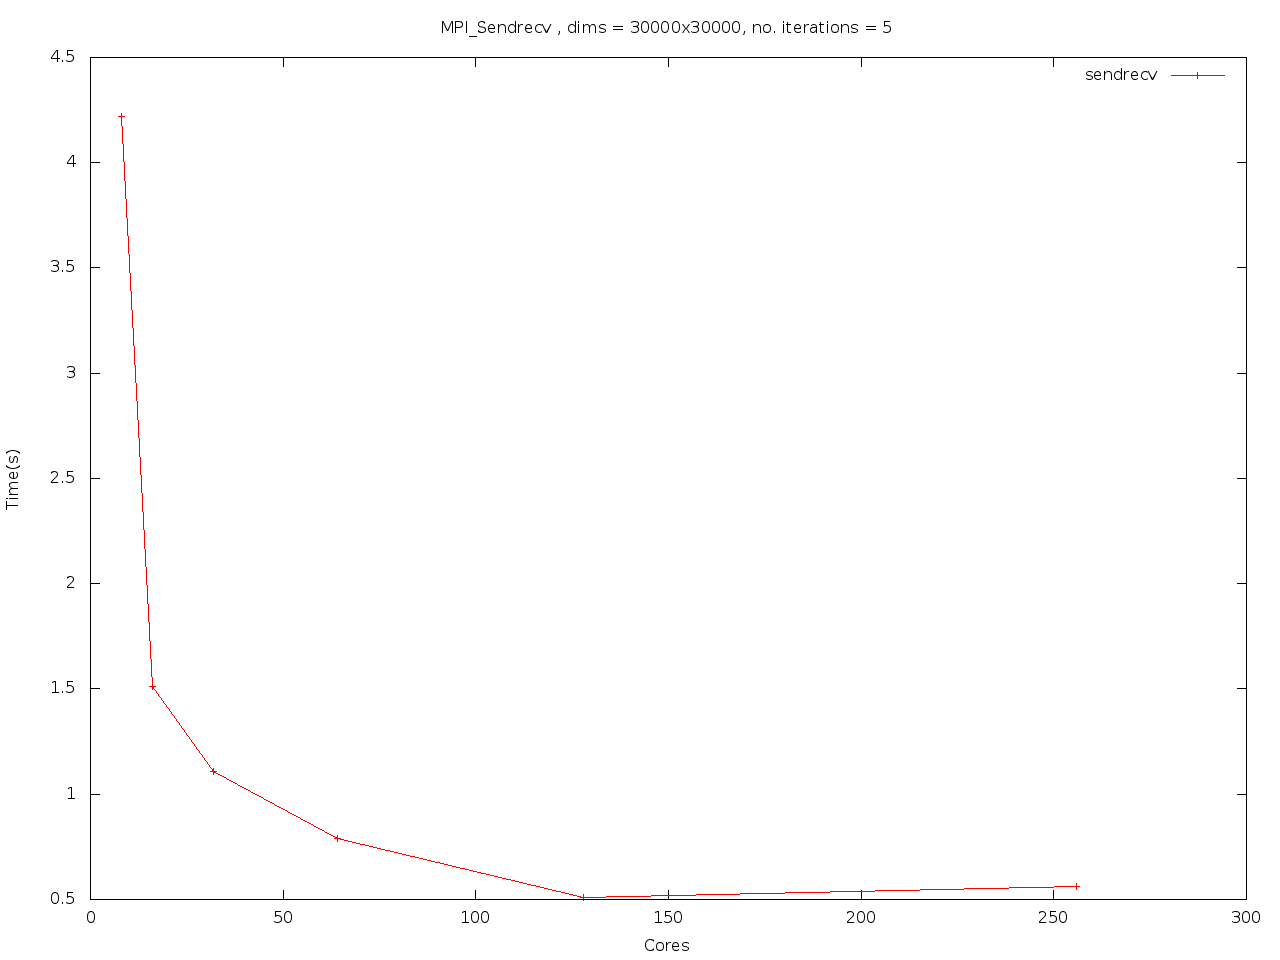
\includegraphics[width=\textwidth]{srcxt.png}

\subsection{Non-Blocking exchange}
The non blocking algorithm works in the same way as the sendrecv implementation, with the only difference that it uses the non-blocking $MPI\_Isend$
$MPI\_Irecv$ for the exchange. We also have to maintain a list of requests for each processor so that we can call MPI\_Waitall.
\begin{lstlisting}[label=some-code, caption=Non-blocking MPI left call + MPI\_Waitall]
      
MPI_Isend (&((*sub_matrix)[1]), 1, col, tmp_rank, 
    1, MPI_COMM_WORLD, &requests[reqs]);
MPI_Irecv (*sub_matrix, 1, col, tmp_rank, 
    3, MPI_COMM_WORLD, &requests[reqs]);

MPI_Waitall(reqs,requests,statuses);

\end{lstlisting}
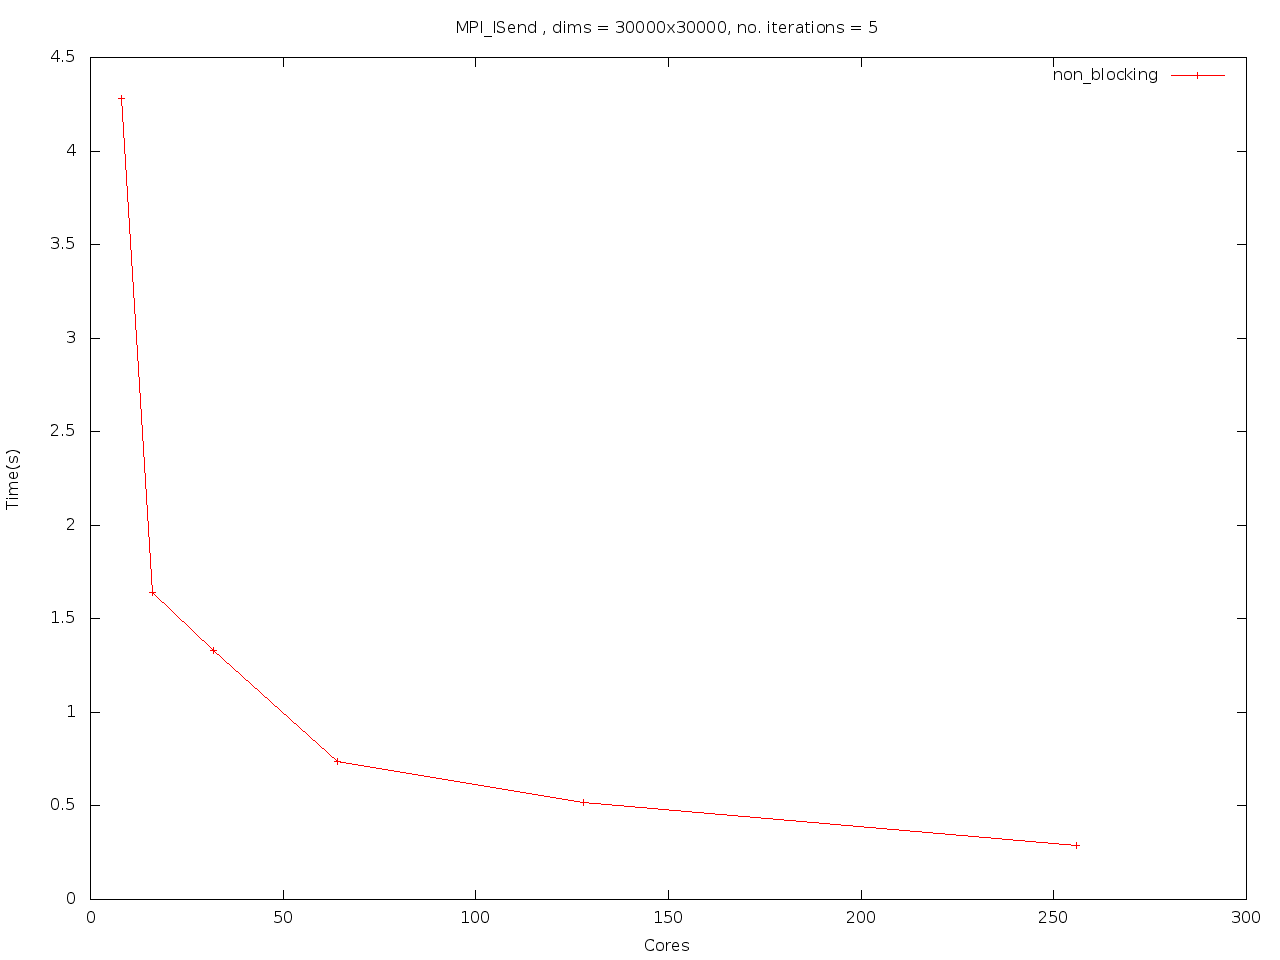
\includegraphics[width=\textwidth]{nbcxt.png}
\subsection{MPI\_Put and MPI\_Get exchange}
Although it was not required, we also implemented a one-sided version of the exchange using MPI\_Get, to test how it would affect the performance 
compared to MPI\_Put. Both programs have to maintain a window for each processor, containing memory for the 4 boundaries of the node. In the case
MPI\_Put, after each put epoch (happening once per iteration) each process needs to copy the new values in the window to its own boundaries. On the
other hand, in the MPI\_Get version after each iteration each process must copy its new updated edges (but not boundaries) to the window. After that
every process gets their new boundaries from the windows of their respective neighours.
\begin{lstlisting}[label=some-code, caption=Left MPI\_Put vs left MPI\_Get call]
      
MPI_Put(&((*sub_matrix)[1]), 1, col, neigh_ranks[get_num], 
    2*SUB_COL + SUB_ROW, SUB_ROW, MPI_DOUBLE, win);

MPI_Get(*sub_matrix, 1, col, neigh_ranks[get_num], 
    2*SUB_COL + SUB_ROW, SUB_ROW, MPI_DOUBLE, win);

\end{lstlisting}

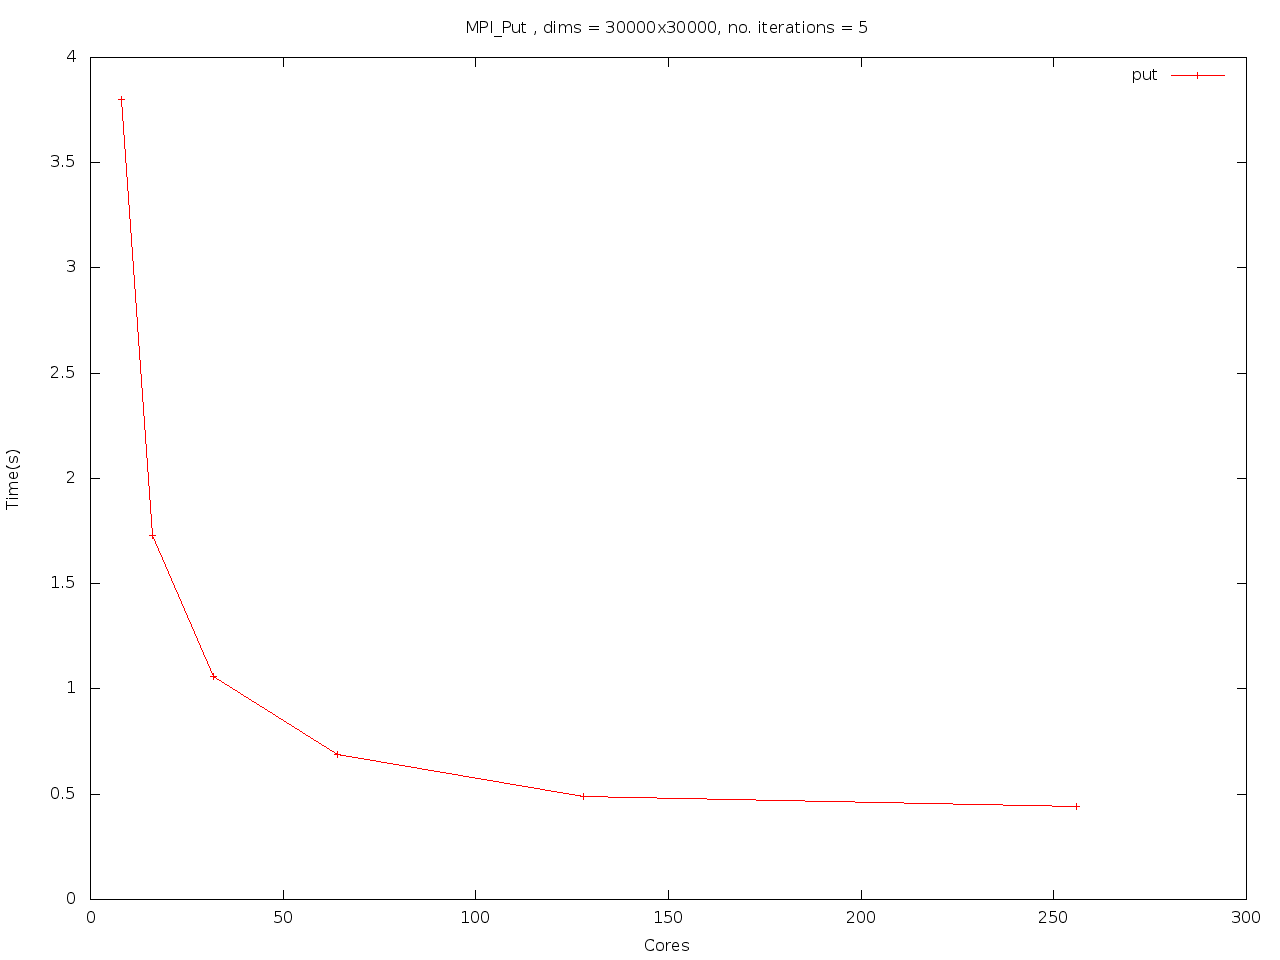
\includegraphics[width=\textwidth]{putcxt.png}
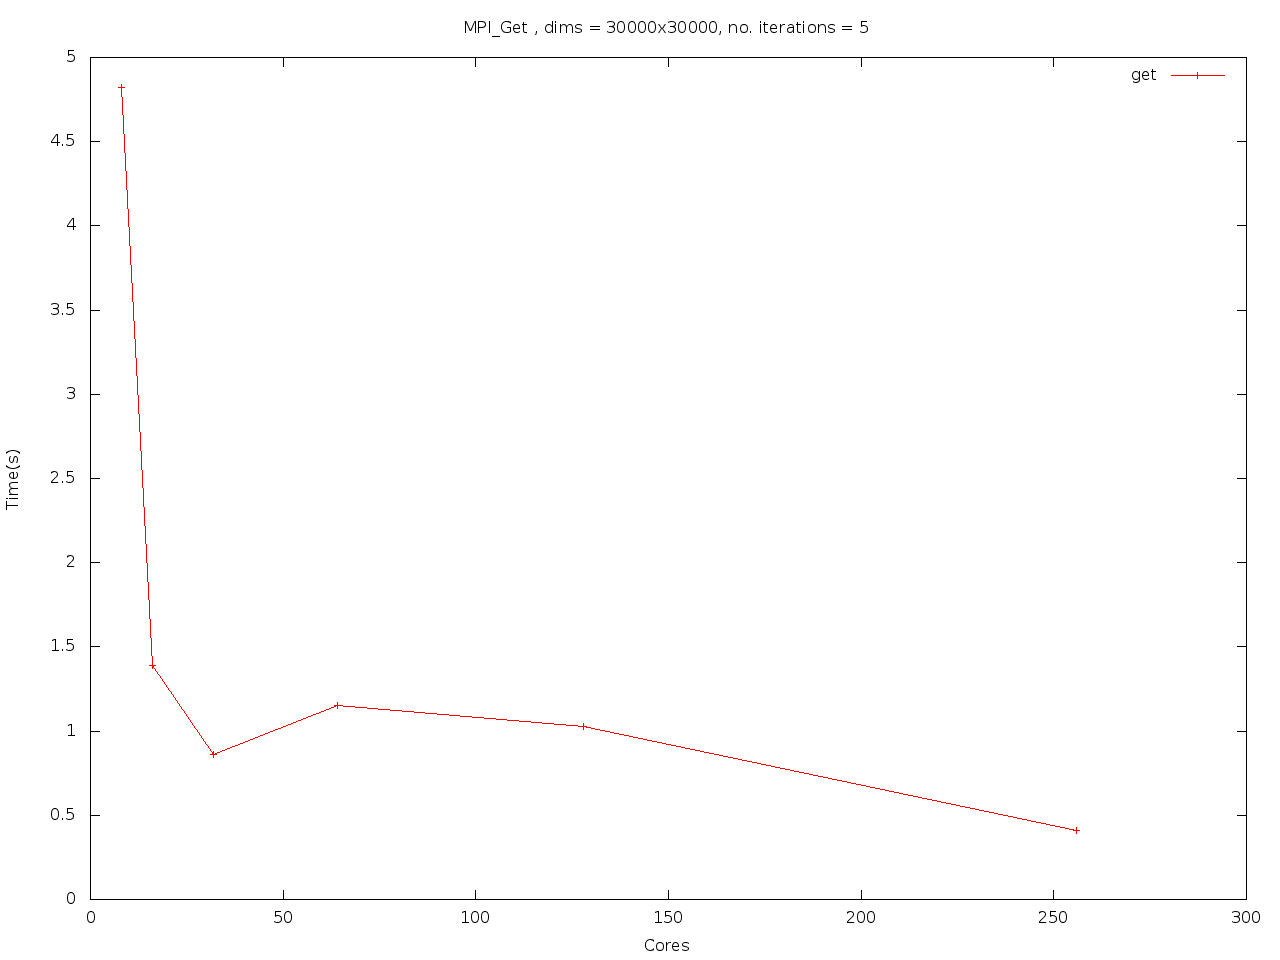
\includegraphics[width=\textwidth]{getcxt.png}

\section{Feedback}
We hope you will enjoy using this release as much as we enjoyed creating it. If you have comments, suggestions or wish to report an issue you are experiencing - contact us at: \emph{http://gummi.midnightcoding.org}.

\section{One more thing}
If you are wondering where your old default text is; it has been stored as a template. The template menu can be used to access and restore it. 

\end{document}
